\documentclass[Nike]{tuberlinbeamer}

\usepackage[ngerman]{babel}  % 'babel' muss geladen werden
\usepackage[utf8]{inputenc}  % optional, aber empfehlenswert
\usepackage[T1]{fontenc}

\usepackage{svg}
\usepackage[export]{adjustbox}
\usepackage{amssymb}
\usepackage{tikz}

% Die ueblichen Angaben
\title{PAVOOC - An AI integrated web-app for CRISPR target recommendation}
\subtitle{Prediction and visualization of on- and off-targets for CRISPR}
\author[Moritz Schäfer]{Moritz Schäfer}
\institute{Technische Universität Berlin \& Bayer Pharma}

% Eigenes Logo einfuegen:
\renewcommand{\pathtomylogo}{meinlogo}

\begin{document}

\begin{frame}
\maketitle
\end{frame}

\section{Motivation}

% Last 8 months in one of these beautiful buildings at Bayer Pharma at Reinickendorfer Straße here in Berlin. There I worked in the oncology department in the target discovery program. But what does this mean?
\begin{frame}
  \begin{figure}
    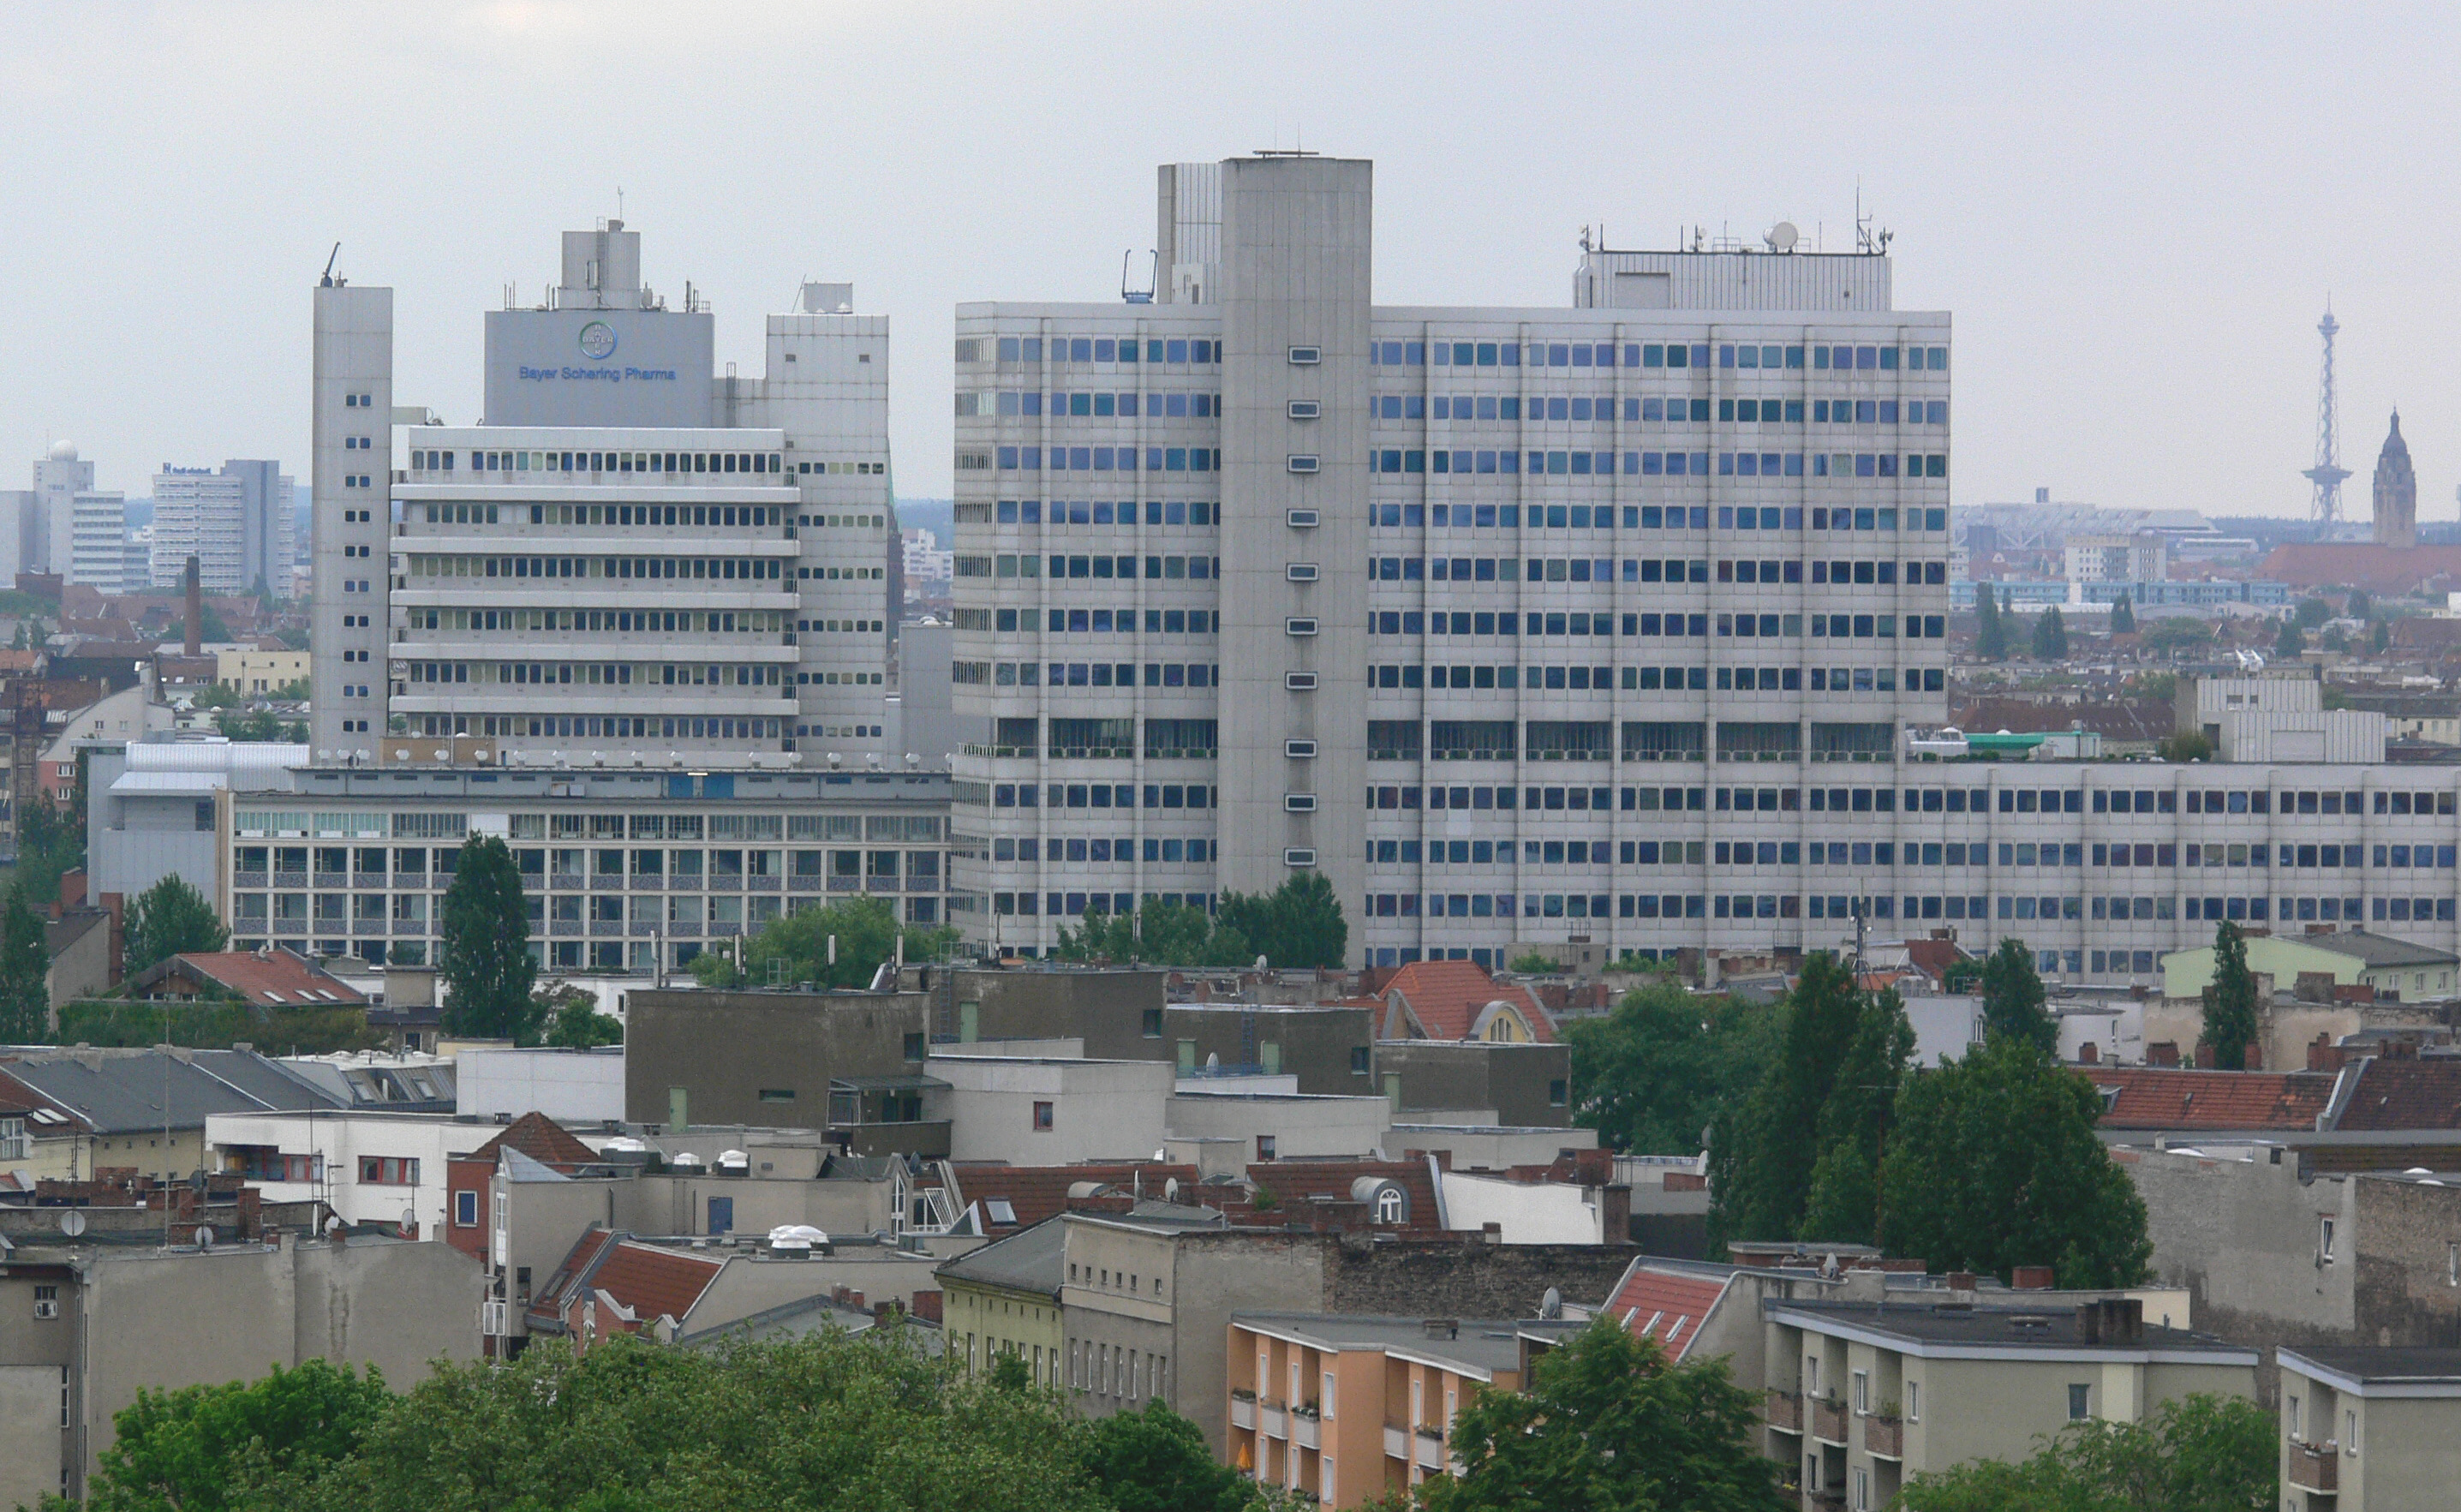
\includegraphics[width=0.9\linewidth]{bayerbuilding.jpg}
  \end{figure}
\end{frame}

% What is Target discovery?
% When talking about cancer research and drug development, or medicine development, a target is a gene which is essential for survival of a cancer cell.
% So we extract a cancer cell from a human or animal, we clone it many many times and then we modify the clones, deactivating one gene at a time. There are around 20,000 genes in humans and we target each of those one by one.
% Now this specific type of tumor cell, like any other cell type, depends on a specific set of genes. If we take out one of these dependent genes, it dies. And this is what we want to achieve.

\begin{frame}{Target discovery}
  \begin{figure}
    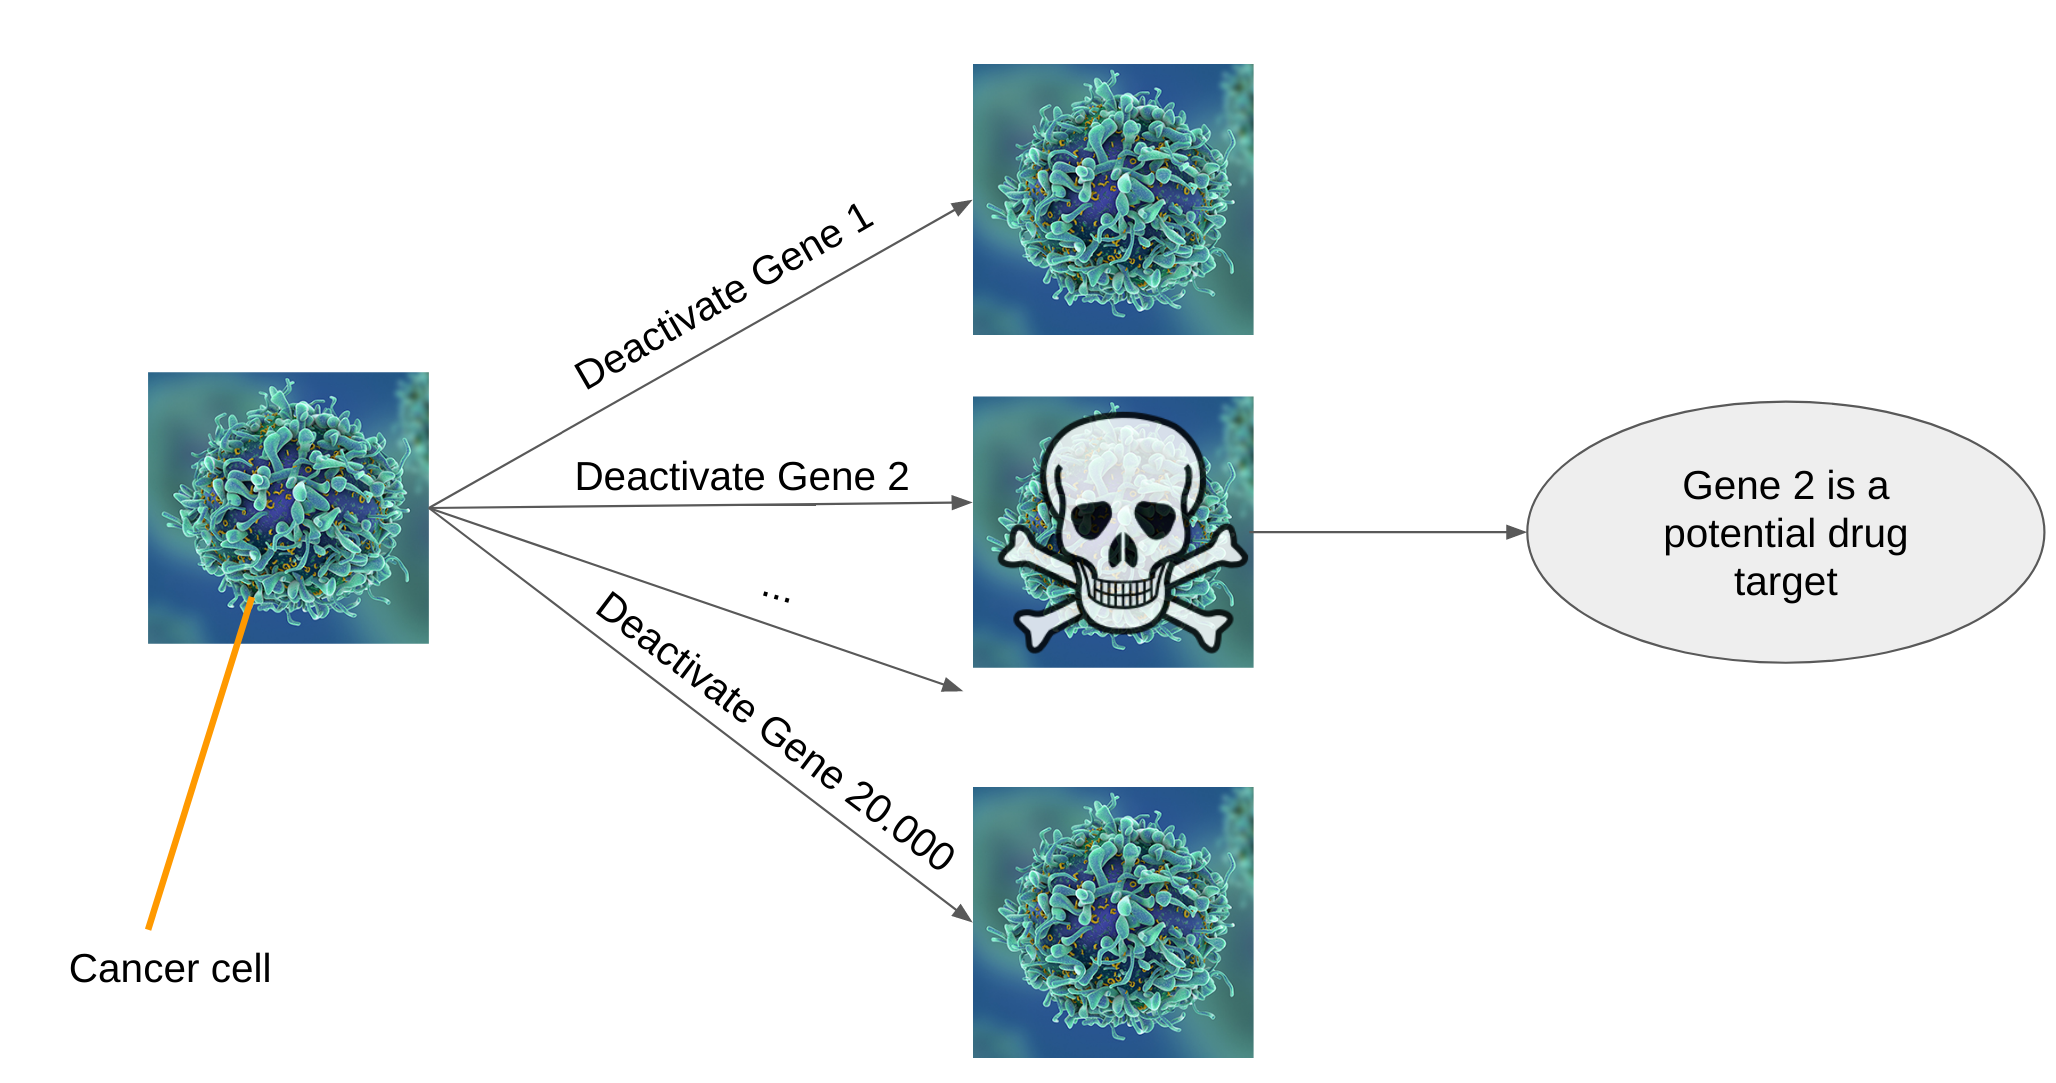
\includegraphics[width=\linewidth]{targetdiscovery.png}
  \end{figure}
\end{frame}

\section{Problem}

% Now this all sounds very promising. Cutting DNA wherever you want, easily disabling specific genes.. However in biology it's never that easy. First of all, the Cas9 protein cuts better or worse depending on the targeted sequence. So if we want to cut inside a gene to knock it out, it can happen, that we target a sequence which is very difficult to cut for this Cas9 protein.

\begin{frame}
  \frametitle{CRISPR problems}
  \begin{itemize}
    \item Guide performance varies significantly
    \pause
    % Another problem arises from the way proteins are being created from the DNA. The amino acids of a protein are coded by triplets of nucleotides in the DNA. The reason why a simple cut in the DNA often results in a knockout of the gene is that this arrangements of thriplets is disturbed. This is called a frame shift and it means, that all subsequent amino acid encodings are changed.
    % In about 30% of all cases however, the random modification introduced here do NOT provoke a frame shift which leads to the modification of several amino acids only.
      \vspace{0.1cm}
    \item Non-frame-shift indels cannot be circumvented
      \includegraphics[width=0.8\linewidth,left]{nonframeshift.png}
    \pause
    \item Cancer mutations may affect binding site
      \vspace{0.2cm}
      \includegraphics[width=0.4\linewidth,left]{guide_snp.png}
  \end{itemize}
\end{frame}

\section{Solution}

% What I did in my master thesis and what I want to show you in this presentation is my solution to these problems. First I designed a machine learning model, which is capable of predicting the likeliness of a guide to cut at the intended site.
% Based on this model, I built a web application, that facilitates the design of CRISPR guides for gene knockout experiments. One key feature of the tool is to enable biologists to circumvent unsuccessful knockouts due to non-frame-shifts

\begin{frame}{Solution}
  \begin{itemize}
    \vspace{0.2cm}
    \item Cutting-edge guide efficacy scoring
      \pause
    \vspace{0.2cm}
    \item Web based guide design tool
      \pause
    \vspace{0.2cm}
    \item Guide filtering for (cancer induced) single nucleotide variations
  \end{itemize}
\end{frame}

% So what I wanna show you here is an overview of the solution I built.
% LIVEDEMO HERE
\begin{frame}{Live Demo}
  \url{https://pavooc.me}
\end{frame}

% As I told before, one large part of my work was to improve the guide efficacy scoring.
\subsection{Guide efficacy prediction}

\begin{frame}{Guide efficacy prediction -- Dataset}
\begin{table}[]
    \centering
    \begin{tabular}{cc}
        \textbf{Guide} & \textbf{Measured efficacy} \\ \hline
\texttt{GTAGGGGTCCGTACTCAGCAAGG} & 0.86 \\
\texttt{ACACTGCCGAGCGATGAGGATGG} & 0.42 \\
\texttt{AAGGTGAAGGAGGATGCGGCGGG} & 0.53 \\
\texttt{GAAAAGATAGGTCACTGACCCGG} & 0.12 \\
\texttt{GCAAGTCACTGAGTGCAGAACGG} & 0.73 \\
\texttt{GCATTGGTAAGCGCACAGGAAGG} & 0.70 \\
\texttt{AAGACTGGCGCATGGTCCACTGG} & 0.57 \\
\texttt{...} & ... \\
    \end{tabular}
\end{table}
\begin{itemize}
  \item 1,837 data rows from 2014
  \item 3,473 data rows from 2016
  \item Efficacy relates to cell proliferation after CRISPR application
\end{itemize}
\begin{flushright}
  \tiny
  ``Optimized sgRNA design to maximize activity and minimize off-target effects of CRISPR-Cas9'', 2016, John G. Doench et al.\
\end{flushright}
\end{frame}

% aus thesis:
% Doench et al. showed in their publications form 2014 to 2016, that CRISPR guide efficacy depends significantly on the sequence of the protospacer.[DHG + 14][DFS + 16] They ran several experiments to determine guide efficacies for different protospacer sequences and built a linear model which considered single nucleotide positions as its inputs.
\begin{frame}{Guide efficacy prediction -- 2014}
  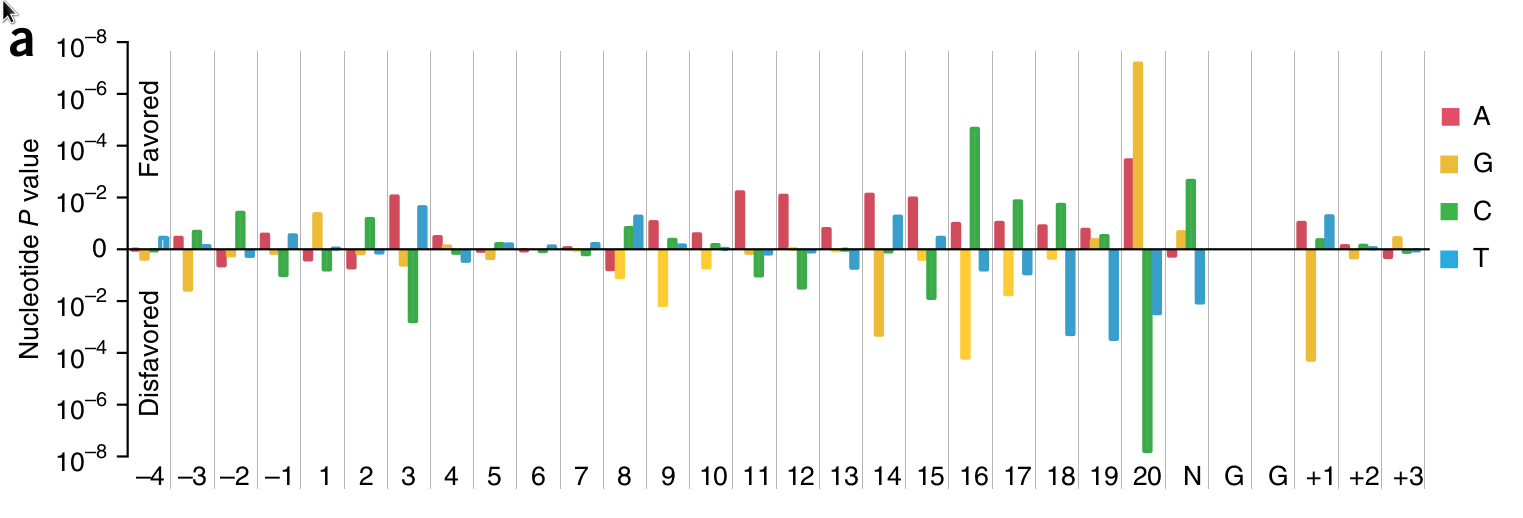
\includegraphics[width=\linewidth]{./nucleotide_table.png}
  \begin{flushright}
    \tiny
    ``Rational design of highly active sgRNAs for CRISPR-Cas9–mediated gene inactivation'', 2014, John G. Doench et al.\
  \end{flushright}
  %What early publications noticed, is that the effectiveness of a guide to a great extend depends on the sequence of nucleotides
\end{frame}

\begin{frame}{Guide efficacy prediction -- 2016 (Azimuth)}
  % Later publications then identified COMBINED adjacent nucleotides as predictive features
  Pairwise nucleotide features

  \pause
  \huge ACTATCTATCGTACGA{\color{red}TT}GA \\
    \pause
  ACTATCTATCGTACGAC{\color{red}AA}G
    \begin{flushright}
      \tiny
      ``Optimized sgRNA design to maximize activity and minimize off-target effects of CRISPR-Cas9'', 2016, John G. Doench et al.\
    \end{flushright}
    \pause
  \center
  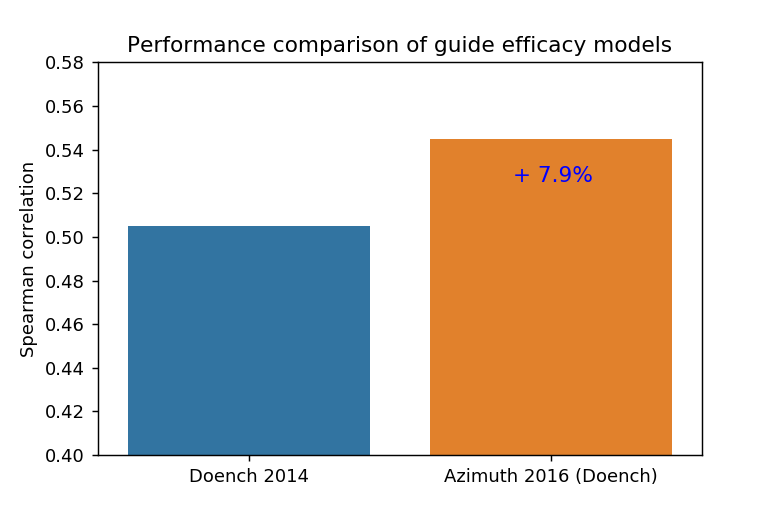
\includegraphics[width=0.5\linewidth]{./model_comparison1.png}
\end{frame}


% Unfortunately, the models they used to identify these combinations only allowed for investigating pairs of nucleotides, though we don't know if three four or more adjacent nucleotides do interact in a way that they influence Cas9 binding.

% To be able to identify such larger combinations, I used a tool called convolutional neural networks
\begin{frame}{Guide efficacy prediction -- Dataset}
\begin{table}[]
    \centering
    \begin{tabular}{cc}
        \textbf{Guide} & \textbf{Measured efficacy} \\ \hline
\texttt{GTAGGGGTCCGTACTCAGCAAGG} & 0.86 \\
\texttt{ACACTGCCGAGCGATGAGGATGG} & 0.42 \\
\texttt{AAGGTGAAGGAGGATGCGGCGGG} & 0.53 \\
\texttt{GAAAAGATAGGTCACTGACCCGG} & 0.12 \\
\texttt{GCAAGTCACTGAGTGCAGAACGG} & 0.73 \\
\texttt{GCATTGGTAAGCGCACAGGAAGG} & 0.70 \\
\texttt{AAGACTGGCGCATGGTCCACTGG} & 0.57 \\
\texttt{...} & ... \\
    \end{tabular}
\end{table}
\begin{itemize}
  \item 1,837 data rows from 2014
  \item 3,473 data rows from 2016
  \item Efficacy relates to cell proliferation after CRISPR application
\end{itemize}
\begin{flushright}
  \tiny
  ``Optimized sgRNA design to maximize activity and minimize off-target effects of CRISPR-Cas9'', 2016, John G. Doench et al.\
\end{flushright}
\end{frame}

%Now the cool thing is, that a convolutional neural networks learns these shapes on its own just be looking at a ton of images. You tell it to classify noses, it will learn filters to detect nose specific shapes.

\begin{frame}{Convolutional neural networks}
  % Let's say we've got 10 guide RNAs which performed really well in a CRISPR experiment. So they all provoked a Double strand break at their target position.
  Well performing guides: \\
  {\large
    GTAGGGGTCCGTACTCAGCA \\
    CAGGGTCCGTACTCAGAGGA \\
    CTAGCGTAGAGCGCACTGCA \\
    ACTGAGCTAGCGTAGAAGCA \\
    TGAGCTAGCGTAGAGCACCA \\
    ACTGAGCTAGCGTAGTAGCT \\
    AGCGTAGAGCGCGCTGCGCC \\
    GAGCGCACTGAGCTAGAGAA \\
    ATAGAGCGCCTGAGCTCGCA \\
    CGTAGAGCGCACTGAGAGCT \\
  }
  % now if you look closely at the last four nucleotides, you notice that they are very similar. A convolutional neural network can recognize this similarity and rerember it with help of a filter.
\end{frame}

\begin{frame}{Convolutional neural networks}
  Well performing guides: \\
  \textcolor{green}{\large
    AGCA \\
    AG{\textcolor{black}G}A \\
    {\textcolor{black}T}GCA \\
    AGCA \\
    A{\textcolor{black}C}CA \\
    AGC{\textcolor{black}T} \\
    {\textcolor{black}C}GC{\textcolor{black}C} \\
    AG{\textcolor{black}A}A \\
    {\textcolor{black}C}GCA \\
    AGC{\textcolor{black}T} \\
  }
  \pause
  Learned filter: \textcolor{green}{[A G C A]}
  % And this is exactly what we want: This filter now helps the neural network to recognize well performing guides
\end{frame}

\begin{frame}{Model architecture}
  \begin{figure}
    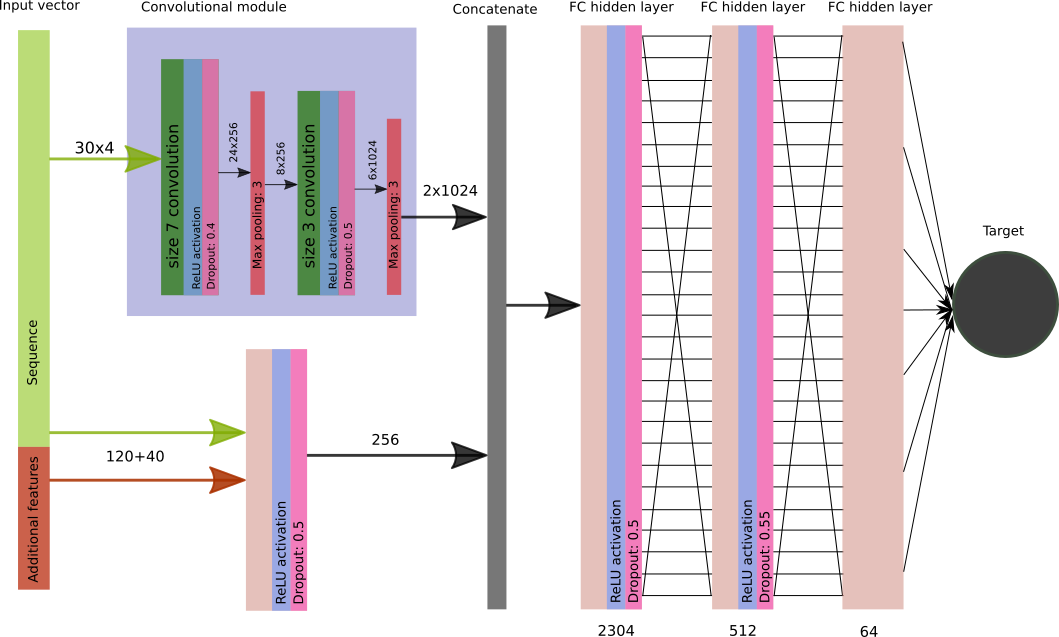
\includegraphics[width=0.65\linewidth]{CNN38_layout.png}
  \end{figure}
  \pause
  \begin{figure}
    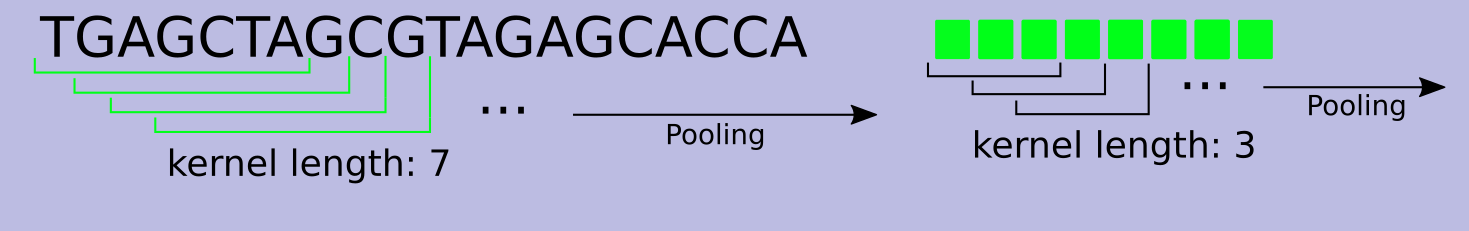
\includegraphics[width=0.65\linewidth]{convolution.png}
  \end{figure}
\end{frame}

% TODO maybe delete
\begin{frame}{Model optimization}
  \vspace{-0.3cm}
  \begin{figure}
    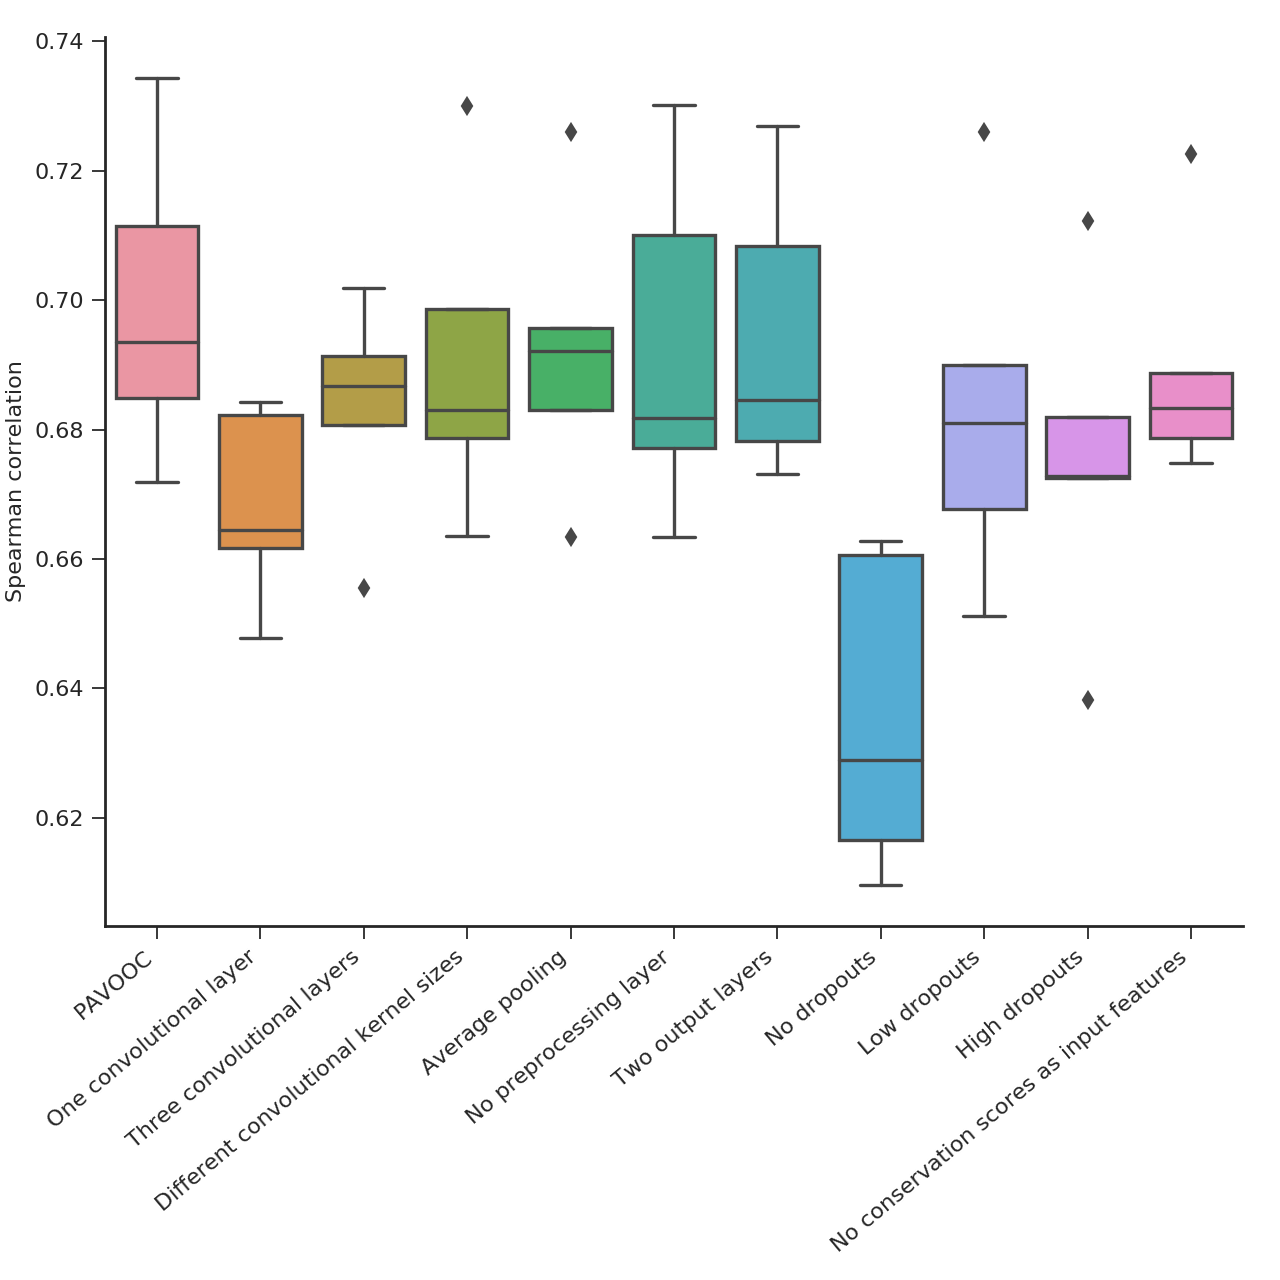
\includegraphics[width=0.57\linewidth]{cnn38_saturation.png}
  \end{figure}

\end{frame}

\begin{frame}{Model architecture}
  \begin{figure}
    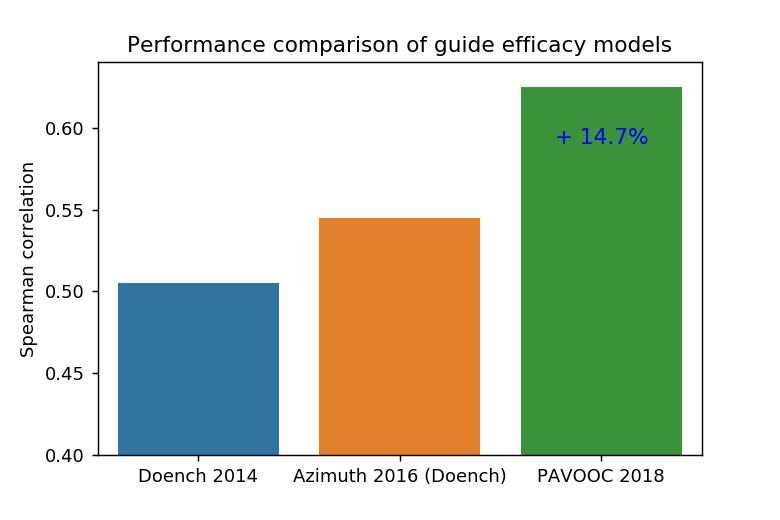
\includegraphics[width=0.65\linewidth]{model_comparison2.png}
  \end{figure}
\end{frame}

% To build the web application, I first developed a data processing pipeline that gathers various relevant data sources, preprocesses them and stores them in an easy to access format in a database. From this data I also generated the BED files being using in the Sequence Browser.
% \begin{frame}{Architecture}
%   \begin{figure}
%     \centering
%     \includegraphics[width=0.65\linewidth]{architecture.png}
%   \end{figure}
% \end{frame}

\begin{frame}{Conclusion and Takeaways}
  % We started with this thought, we achieved this in the end
  \begin{itemize}
    \item PAVOOC provides amino acid level bindings
    \item Cas9 efficacy depends on complex biological coherences % which is why a more complex model boosts performance
    \item DL improves guide efficacy prediction %
    \item DL feasible with \textasciitilde5,000 rows
  \end{itemize}
  Disclaimer: My model is not employed in the website for publication reasons.

\end{frame}
%% end %%


\begin{frame}{Future Work \& Discussion}
  \begin{itemize}
    \item Additional input features (chromatin accessibility)
    \item Evaluate model on different datasets
    \item Support additional species and assembly versions
  \end{itemize}
\end{frame}

% At this point it's probably a good idea how the performance of a model is evaluated for such a problem. The Spearman correlation coefficient is the de facto standard for guide efficacy prediction. In contrary to the linear Pearson correlation it is based


\begin{frame}{Performance evaluation}
  \begin{figure}
    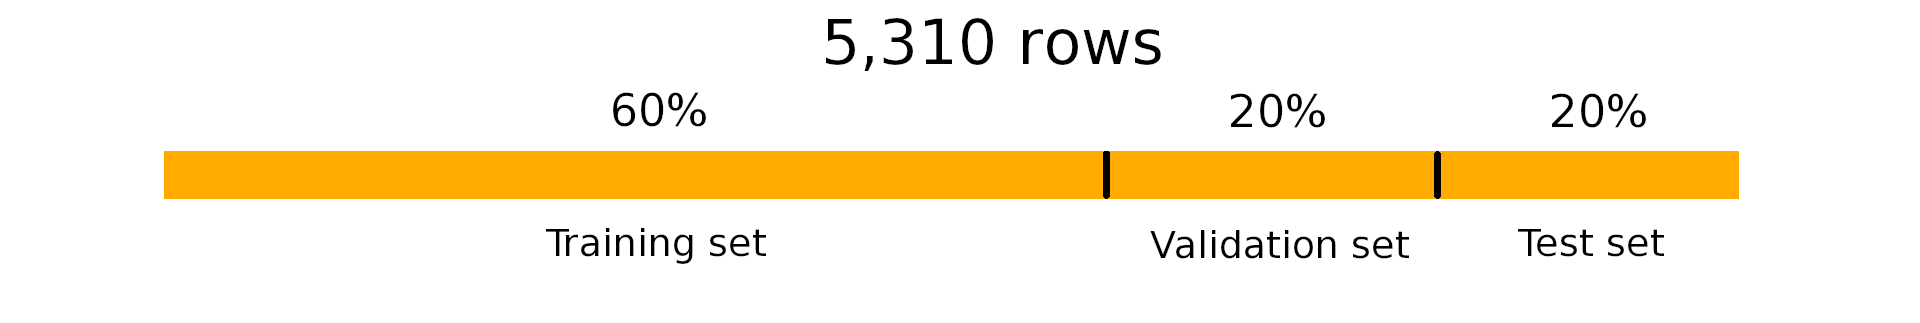
\includegraphics[width=0.60\linewidth]{./datasetpartition.png}
  \end{figure}
  \pause
  \begin{figure}
    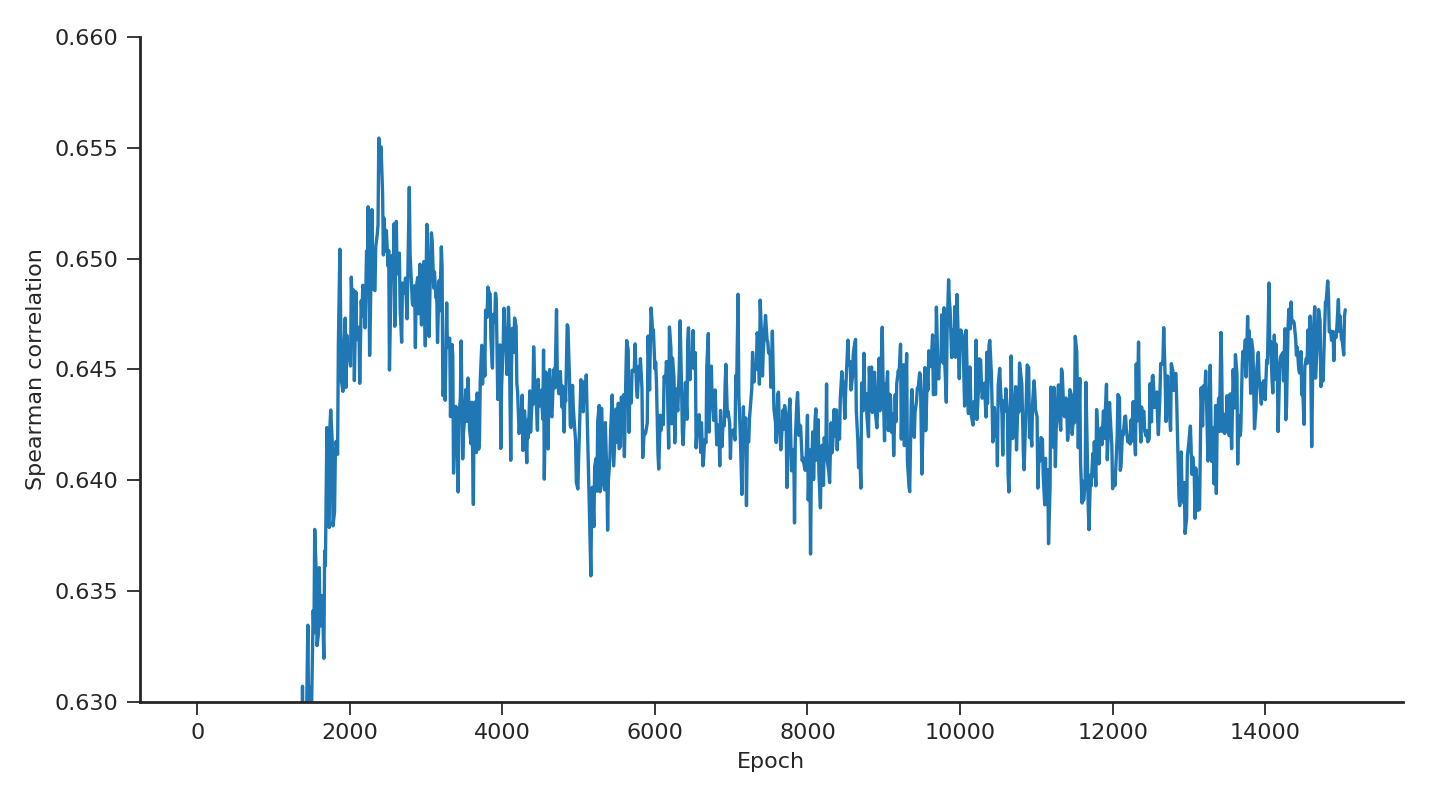
\includegraphics[width=0.75\linewidth]{./validation_training_curve.png}
  \end{figure}

\end{frame}


\end{document}
